
\documentclass[letter, 9pt, conference]{ieeeconf}

\IEEEoverridecommandlockouts

\overrideIEEEmargins

\usepackage[utf8]{inputenc}
\usepackage[T1]{fontenc}
%\usepackage[top=0.75in, bottom=1in, left=1in, right=1in]{geometry}
\usepackage{xcolor}
\usepackage{graphicx}
\usepackage{url}
\usepackage{float}
\usepackage{hyperref}
\usepackage{minted}
\title{LINGI2142: Computer Networks \\ Transit Network Simulation}
\author{\textsc{Langlois Quentin} - 19281700 \and \textsc{Dardenne Florent} - 02601700 \and \textsc{Iavarone Simon - 29911700 }}


\begin{document}

\maketitle
\thispagestyle{empty}
\pagestyle{empty}


%%%%%%%%%%%%%%%%%%%%%%%%%%%%%%%%%%%%%%%%%%%%%%%%%%%%%%%%%%%%%%%%%%%%%%%%%%%%%%%%
\begin{abstract}

This report describes our analysis of the European OVH network topology. It details different aspects such as OSPF, BGP, security and anycast. In the end, we present our simulation techniques, tests and results. 

\end{abstract}


%%%%%%%%%%%%%%%%%%%%%%%%%%%%%%%%%%%%%%%%%%%%%%%%%%%%%%%%%%%%%%%%%%%%%%%%%%%%%%%%
\section{Introduction}

As part of the computer networks course \cite{LINGI2142}, we were asked to choose a part of the OVH network, describe and emulate it with the IPMininet \cite{ipmininet} library.

The objective of this project is therefore to discover how BGP works in a network by configuring it in the best way, to discover and implement BGP communities, to support the anycast protocol and to improve the network security. In order to get the most out of it, we will no longer consider OVH as a service provider but as a transit network.

This report will first describe the area of the OVH network we have chosen as well as our strategy in this network for the implementation of the BGP and OSPF protocols.

Then we will present our strategy and implementation of 3 additional aspects such as the security, the BGP communities and the anycast protocol. 

Finally, we will show our simulation methodology, tests and results. 

\section{Description of the topology}

\subsection{Zone description}

We chose the European zone of the OVH \cite{OVHweathermap} topology. This choice was made for 2 reasons : 

\begin{itemize}
    \item There are many redundancies in this part of the network. 
    \item Many external ASes are present at many places which allows us to explore in more details the eBGP mechanism. 
\end{itemize}

\begin{figure}[H]
    \includegraphics[width=\linewidth]{topo_schema.jpeg}
    \caption{Topology representation}
    \label{fig:topo_schema}
\end{figure}

Legend : 
\begin{itemize}
    \item Boxes represent routers and their color represents their AS (one color per AS). 
    \item Links represent physical links with their associated IGP cost\footnote{See section \ref{sec:ibgp} for more details} (1 by default). 
    \item Circles represent a group of Route-Reflectors. 
\end{itemize}



\subsection{OSPF and addressing plan}
\label{sec:ospf}

In order to save a maximum of IP addresses, we made an hierarchical addressing plan. 

For this purpose, we first assigned a specific subnet for each AS (in /24 for IPv4 and /48 for IPv6). 

Next, we divided the OVH network by region (cities) and gave them a more specific subnet (in /28 for IPv4 and /56 for IPv6). 

The last step was to determine the loopback-address of routers and the address of their interfaces for link addresses. As described in the section \ref{sec:simulation}, we made an incremental address generator for loopback-address and used the same technique for link-addressing. \\
This means we took the first available address (in /32 or /128 for loopback) and assigned it to the router. For the links, we chose the subnet of one of the two routers and generated 2 addresses (in /31 or /127) in order to put the 2 routers in the same subnet. 


\subsection{iBGP configuration}
\label{sec:ibgp}

In order to have a minimal number of iBGP connections, we made a multi-level Route-Reflector (RR) architecture. In this type of architecture, low-level RR are clients of high-level RR.

Furthermore, as shown in Fig. \ref{fig:ibgp_schema}, the iBGP connections follow, in most cases, physical links connections. 

In order to create redundancy, all routers are connected to at least two Route-Reflectors. 

IGP costs allow to avoid diflection also in case of crashes. 

\begin{figure}[h!]
    \includegraphics[width=\linewidth]{ibgp_schema.jpeg}
    \caption{iBGP connections}
    \label{fig:ibgp_schema}
\end{figure}

Description of the RR-levels : 
\begin{itemize}
    \item \textbf{First level} : main level which will dispatch routes to second-level-RR. \\
    We chose \textit{fra-5} and \textit{par-gsw} because they are connected to many other ASes and therefore have a central position and receive many external routes. 
    \item \textbf{Second level} : we splitted the second-level RR in 2 sub-groups:
    \begin{itemize}
        \item At the left of the topology, \textit{milan} and \textit{sbg-g1}, will dispatch routes to this part. 
        \item \textit{ams-5}, \textit{vienne} and \textit{varsovie} which will dispatch routes to the left part of the topology. 
    \end{itemize}
    A fullmesh is done for each subgroup. 

    \item \textbf{Third Level} : This level of RR is specific to the Anycast part of the simulation. We will therefore consider it later in the anycast simulation section.
\end{itemize}

\subsection{eBGP configuration}
\label{sec:ebgp}

In order to have a more realistic topology, each external AS router for each eBGP connection with OVH are different. Actually, one unique router connected to Milan, Warsow, Amsterdam, Paris and Frankfurt for the UPC AS seemed not realistic at all. 

IPMininet creates several import/export route-maps depending on the type of eBGP link. Unfortunately these different route-maps interfere with our BGP communities policy. In order to implement our communities correctly, we therefore decided to consider all external AS as customers (technically, we set the eBGP session to None in IPMininet). However, we are aware that a transit network does not only include customers but also suppliers and peers. 

\subsection{Topology summary}
\label{sec:summary}

As described in section \ref{sec:simulation}, we also added methods to print statistics on the topology. Here is a screenshot of the result. 

\begin{figure}[h!]
    \centering
    \includegraphics[width=0.90\linewidth]{config.png}
    \caption{Information about the topology}
    \label{fig:topo_summary}
\end{figure}


\section{Security}
\label{sec:security}

\subsection{Security techniques}

In a first part we will discuss all the security aspects we thought of implementing. All these aspects are covered in lots of detail in Ref. \ref{src_sec}. We will shortly describe all the techniques of the article. We have not tried to implement them all, but we believe it might be interesting to present them here. \\

The first security technique we will cover is the GTSM (Generalized ttl security mechanism). To implement this technique we have to ensure three things. 
If one of our routers that has an eBGP connection receives a packet with ttl < 255 then it must drop it.
All the packets that are sent by our routers on the bgp port (port 179) should have their ttl set to 255.
Furthermore, we must force our eBGP neighbors to follow the aforementioned rule.

Another security guideline is to use MD5 to ensure that only peers with whom we have an agreement will transmit data to our network. To enforce this policy we have to establish a secret and we have to communicate it to the peer. We tried to implement both these techniques but were not successful. We will describe what was tried later. \\

Another technique that is recommended is prefix filtering. The article mentions two sources that contain all the special prefixes and instructions on how to route them in ipv4 and ipv6. Furthermore, we must avoid forwarding packets to addresses that were not allocated by the IANA. This idea does not make sense in ipv4 anymore but can be useful in ipv6. It is important to note that this aspect must be updated when the IANA allocates new prefixes. \\

Maximum prefixes on a peering. The idea of this technique is to set a threshold on the number of prefixes we receive from a peer. By doing this, we ensure that nobody will send us the whole internet's routing table as it would be quite annoying. 

Another way to secure your network from the outer world is by filtering the AS-Path. One of these rules is to ensure that the first AS number in the AS-Path of the packet is the AS number of the AS the packet comes from. We should then ensure that the packets sent by our AS contain an AS-Path that is not empty. 

The last discussed technique is the filtering of the bgp nexthop. The way to implement it is to check that the bgp nexthop of a router is his bgp neighbor.

\subsection{Security simulation}
\label{sec:security}

This section will just describe the security aspect of the simulation. Other aspects will be discussed in Sec. \ref{sec:simulation}. 

We first tried to implement the GTSM. We tried inserting FRrouting commands in the bgpd.mako file in ipmininet but were not successful. There is indeed an FRrouting command that should activate the GTSM mechanism and another one that should handle the secret sharing for md5. When we tried adding these commands, pingall in our topology would drop dramatically.     

The second thing we tried is using IPTables in python. At first we tried to insert the rule manually. This worked fine.
\begin{figure}[H]
    \centering
    \includegraphics[scale=0.355]{iptables.PNG}
    \caption{}
\end{figure}

But then we had problems figuring out how to insert these kind of rules in python. When we simply created the rule and then proceeded to add the IP(6)Tables daemon the code would not work. We have just upgraded the kernel on the machine and it seems to work right now : 
\begin{figure}[H]
    \centering
    \includegraphics[scale=0.355]{iptablesrouteur.PNG}
    \caption{}
\end{figure}

Now after having upgraded the system, IPTables seem to be working fine. From now on it should be fairly easy to set more IPTables rules. You can find the topology that was used in the file \texttt{project\_tests/security\_topo.py}.


\section{BGP communities}
\label{sec:communities}

\subsection{BGP Communities techniques}

 The BGP protocol defines attributes to influence the routing of packets in the network. Among these attributes we find the local-pref, the AS-Path, the MED, etc. In this section we are interested in the communities attributes. BGP communities are attributes allowing to group several routes in a single entity where the same routing decisions can be applied \cite{obo_communities}.

We have defined in the transit network several communities with each time a different strategy. To describe these different types of communities we will use the classification defined by Quoitin and Bonaventure \cite{obo_quoitin}:

\begin{itemize}
    \item \textbf{Inbound communities}: 
    
    \begin{itemize}
        \item Set local-pref: We have implemented communities allowing customers to modify the local-pref of their routes in the transit network. These allow them to define priority and backup routes. The MED also allows them to do this, but since the local-pref is located before the AS-Path in the BGP decision, it is important in certain situations.
        
        \item Route-tagging: We decided not to include route-tagging communities because we do not consider them useful in the network. Furthermore we avoid to create too many communities as much as possible because they increase the size of our BGP messages and can induce unnecessary updates  \cite{impact_communities}.
    \end{itemize}
    
    \item \textbf{Outbound communities}: These communities allow to filter BGP announcements and allow modifying other attributes in the route when redistributing routes in order to do traffic engineering.
    
    \begin{itemize}
        \item Announcement:  We provide customers with communities to filter their route announcements from the transit network to other customers in certain cities. 
        
        \item AS Prepending: These BGP communities allow customers to request the transit network to prepend the transit network AS in the AS-path x times when a router announces it at the eBGP level to a customer. This community allows client AS to indicate their preferences to other AS in relation to the different transit network of which they have a BGP session. 
        e.g. if Google prefers to be contacted via AS3-transit rather than AS4-transit then it will request an AS-path prepending to AS4-transit to have a higher AS-Path than AS3-transit.
        
        Not having been able to do it in time we could not implement it in our topology. However, it would be an interesting community to know how to implement it even if in our topology its usefulness would be quite limited.

    \end{itemize}
    
    \item \textbf{Blackhole}: Blackhole communities allow AS to ask their ISPs to block certain packets. It is a community of interest for security and especially for dealing with DoS attacks.
    We have not implemented it in our transit network. 
    
\end{itemize}

\subsection{BGP Communities in our topology}

In the table below we can see the communities we have created in our transit network and their action. 
\begin{table}[h!]
\centering
\begin{tabular}{|l|l|}
\hline
Community & action                                                                                                                         \\ \hline
16276:120 & Set local-pref to 120                                                                                                          \\
16276:90  & Set local-pref to 90                                                                                                           \\
16276:80  & Set local-pref to 80                                                                                                           \\
16276:401 & Do not announce to customer in Paris                                                                                           \\
16276:402 & Do not announce to customer in Amsterdam                                                                                       \\
16276:403 & Do not announce to customer in Vienne                                                                                          \\
16276:404 & Do not announce to customer in Frankfurt                                                                                      \\
16276:405 & Do not announce to customer in Varsovie                                                                                        \\
16276:406 & Do not announce to customer in Roubaix                                                                                         \\
16276:407 & Do not announce to customer in Prague                                                                                          \\
16276:408 & Do not announce to customer in Milan                                                                                           \\
16276:409 & Do not announce to customer in Strasbourg                                                                                      \\
16276:410 & Do not announce to customer in Zurich                                                                                          \\
16276:20x & \begin{tabular}[c]{@{}l@{}}Prepend x times the AS in the AS-Path \\ when announcing to customer (not implemented)\end{tabular} \\ \hline
\end{tabular}
\label{table:communities_table}
\caption{BGP Communities implementation}
\end{table}

\subsection{BGP Communities in our simulation}

In this part we discuss how the implementation of this part was done in our code.\\

In order to create route-maps to implement the set local-pref we had to modify the IPMininet library. Indeed, this one unfortunately didn't give us enough flexibility to do it. \cite{issues}
By adding some parameter to the function, we managed to implement the local-pref and provide it to the transit network customer. We will see in the sub-section "Test" and "Result" the customers using this functionality.\\

For the outboud announcement functionnality it was easier, the technique here was to use the deny function of the IPMininet library with the name of a route-maps already created by IPMininet and an order smaller than this one. We will also see in the sub-section "Test" and "Result" the customers using this functionality.  \\

Finally the implementation of these features required a lot of route-maps debugging in the router configuration. This allowed us to understand in depth how route maps work.






\section{Anycast}
\label{sec:anycast}

\subsection{Anycast techniques}

Anycast is the ability to have multiple \textbf{servers} with the same IP address in a network and join the nearest one from its position. 

There are many possible utilization for this feature such as DNS servers, data-centers, ... 

In order to configure anycast, there are 3 main methods : 
\begin{itemize}
    \item \textbf{DNS zones} : grouping some servers under a unique domain name. 
    \item \textbf{OSPF} : advertise multiple times the same IP address over OSPF. 
    \item \textbf{BGP} : advertise multiple times the same IP address over BGP. 
\end{itemize}

\subsection{Anycast in our topology}

For this project, we chose the third solution : anycast over BGP. \\
Here are some reasons : 
\begin{itemize}
    \item The implementation is pretty easy. 
    \item The BGP decision process allows to advertise the route to the nearest server. 
    \item The convergence in case of failure is relatively fast. 
    \item It allows to use BGP properties such as communities to make traffic engineering. 
    \item It allows to better secure the server's behaviour compared to the OSPF technique. 
\end{itemize}

\subsection{Anycast in our simulation}

More details about the simulation are given in its appropriate section. We will just show here the anycast aspect of it. 

As we chose the BGP method to implement anycast, the simulation was easy to implement because BGP is well supported by the ipmininet library. 

However, the BGP daemon is not supported by the \textbf{Host} class and we therefore chose to use the \textbf{Router} class to represent anycast servers. 

To specify their common anycast IP address, we just specify it as their loopback-address. 

In order to advertise this anycast address to other AS, we had to connect these anycast servers to a Route-Reflector. To simplify the simulation, we added a new level of Route-Reflector responsible to advertise anycast server's routes\footnote{if their neighbor router was already a RR, we just added the anycast server to its clients.}. 

\section{Simulation}
\label{sec:simulation}

\subsection{JSON representation}
\label{sec:json}

For the project, we chose to create an automatized construction of the topology based on a structured representation of it. One of the easiest and most common way to structure data is the \textbf{JSON} format. 

Here is a brief overview of our formatted OVH topology and its different configuration fields :

\begin{minted}{python}
{
# subnets to infer loopback and links addresses
  "subnets" : {
    "net_ovh" : { # Main OVH subnet in /24 and / 48
      "ipv6" : "beaf:cafe:babe:/48",
      "ipv4" : "204.32.46./24"
    },
    "net_mil" : { # Specific subnet in /28 and /56. 
      # Adresses are structured with the 
      # 'net_ovh' field. It will be replaced
      # by the corresponding address of this subnet
      "ipv6" : "{net_ovh}0500::/56",
      "ipv4" : "{net_ovh}112/28",
      "nodes" : ["milan"]
    },
    # ... other subnets for the cities
    "net_upc" : { # Example of subnet for another AS. 
      "ipv6" : "beaf:cafe:bab1::/48",
      "ipv4" : "204.32.48.0/24",
      "nodes" : ["upc_var", "upc_vie", ...]
    },
    # ... other subnets for ASes
  },
  "AS" : {    # ASes in the topology
    "OVH" : { # Our main AS. 
      # Routers in the AS with their configuration. 
      "routers" : {
        #As milan has a 'clients' field, 
        #it is considered as a RR. 
        "milan" : { # Name of the router : milan
          #Peers, clients and level for the RR
          #Note: if level is not specified,default=1
          #peers should only be specified for level>1
          "clients" : ["zurich", "sbg-g2"],
          "peers" : ["sbg-g1"],
          "niveau" : 2
        },
         #Simple router without config:
        "zurich": {},
        # ... other routers
      },
      # Default config for all routers of
      # this AS
      "rconfig" : {
        "daemons" : {   # Default daemons
          # Daemons without config:
          "ospf": {}, "ospf6":{},
          # Config for the BGP daemon:
          "bgp": {    
            "communities": {
              # Communities to add
              "set_local_pref": {
              # Conditionned Local-pref
                "16276:120": 120
              }
            }
          }
        }
      },
      "anycast" : [ # Anycast servers in this AS
        {
          "addresses" : { # Anycast addresses
            "ipv4": "10.10.10.10/32", 
            "ipv6": "10::10/128"
          },
          # Nodes to which connect an 
          # anycast server
          "nodes" : ["milan", "varsovie", "ams-1"]
        }
      ]
      # the field 'hosts' can also be added 
      # to specify hosts in the AS
      # In our case, we did not have any hosts 
      # so this field is not present. 
      # However, for our tests, we added many 
      # fictitious hosts automatically
    },
    "Telia" : {
      "routers" : { ... },
      "rconfig" : {
        # Daemons are specified
        # as a list (no config)
        "daemons" : ["ospf", "ospf6", "bgp"]
      },
      # Automatically create a fullmesh of links
      # between all routers of the AS
      "linked" : true
      # Automatically create a iBGP fullmesh
      "bgp_fullmesh" : true
    },
    # ... other AS configuration
  },
  "links" : {   # Physical links
    "milan"    : [  # Node and its neighbors
      "zurich",   # Link without config
      # Link with specified IGP metric
      ["sbg-g1", {"igp_metric": 4}],
      ["sbg-g2", {"igp_metric": 4}]
    ],
    # ... Other links
    # Example of a link between routers from 
    # 2 different AS. 
    # The code will automatically create an 
    # eBGP connection between them
    "amazon_par"  : ["par-th2"]
  }
}

\end{minted}


\subsection{Topology generation}

In this section, we will briefly describe the main aspects of the topology generation that are useful to understand our tests. 

A more detailed description of each part of the construction (AS, routers, links and subnets) can be found on our code. 

\subsubsection{IP address generator}

In order to easily generate IP addresses, we created an IP address generator based on a specific subnet. This generator is used in 2 features : loopback-address and link-address generation. 

For the loopback-address part, the target is to create a /32 (or /128) address based on the router's subnet. As shown in the section \ref{sec:json}, we can easily get the subnet of a specific router. \\
After the identification, we compute the number of already created addresses for this subnet, add 1 to the last byte and obtain the new address. 

For the links-addresses, the difficulty was to create a /31 (or /127) address so we had to determine the right subnet (and not add 1 like for loopback addresses). \\
To solve this, we computed the next multiple of 2 ($ 2^{32 - 31} $) for the last byte and it gives us the first address of the subnet. We then compute the second address by adding 1 to the last byte. \\
\textbf{Note} : to select the subnet for the link, we took the subnet of the link's "main"\footnote{The main note is the key in our json-format of links. The values are its neighbors.} node.

\subsubsection{Hosts generator}

In order to make tests on our topology (ping, traceroute) we also provided a tool to add fictitious hosts to AS\footnote{A more detailed description of the different features of this tool can be found in the documentation of our \textit{JSONTopo class}}.

As a basic usage, we simply added 1 host for each router of each AS. With this technique, we were able to test connections between all parts of our topology. 

\subsection{Tests}
\label{sec:tests}

For our tests, we used the \textbf{Mininet command-line} to execute commands on our routers. Here is a brief overview of commands used to test different aspects : 

\begin{itemize}
    \item \textbf{OSPF and BGP} : as shown in the previous section, we added many fictitious hosts in our topology. This allowed us to test the connectivity between all pairs of routers with the \textbf{ping6all} command. We also verified through the \textbf{traceroute} command that the path taken by each host to other hosts was in accordance with our expectations.
    \item \textbf{Security} : To test our security topology we used the pingall, ping6all, iptables and ip6tables commands
    
    \item \textbf{BGP communities} : In order to test our communities, we have had external AS attach communities to their roads.\\
    
    \begin{itemize}
        \item The Set Local-pref test : 
        
        Level3 router in Frankfurt attaches community 16276:120 to its routes towards our network. This community allows it to define the local-pref of its routes at 120 : this will be its main link.\\
        Then it is the level3 router in Frankfurt which attaches the community 16276:80 to set the local-pref of its routes to 80 : this will be the backup link of the AS level3.\\
        
        In order to test this, we first look if the route-maps are correctly defined in the routers. Then we perform traceroutes from routers to level3 to make sure that only the link to Frankfurt is used. Finally we cut the link between Level3 Frankfurt and our network to see if the backup link Level3 Paris is used correctly. We will see the results of this test in the next section.\\
        
        \item The Outbound Announcement test:
        
        UPC does not wish to announce its routes to the transit networks customers located in Paris. For this purpose it will attach the 16276:401 community to its routes.\\

        In order to test this, we will make a ping between Amazon AS which is only attached to Paris in our network and UPC. If our community works well, Amazon being isolated in Paris, it will not be able to contact UPC and vice versa. UPC will know the route to Amazon but Amazon don't know the route to UPC so it can't answer to it.
        To be sure that it is not a firewall blocking the pings, we will check in Amazon's routing table that the routes to UPC are not there.
        
        
    \end{itemize}

    
    \item \textbf{Anycast} : in order to test Anycast, we added 3 anycast-servers in different places (cf section \ref{sec:json}, anycast entry). Next, we used the traceroute command from different hosts (inside / outside our AS) to the anycast address and see which server has been reached. 
\end{itemize}

\subsection{Results}

\paragraph{OSPF and BGP results} with the \textbf{ping6all} command, all hosts tried to contact each other hosts so that we could check if all parts of our network is reachable by all other parts. The result of the command showed a 0\% packet drop : it means that all routes are well distributed and reachable in the whole topology. \\

We then traced the paths taken by some hosts to other hosts and then checked with \textbf{traceroute} if they were in agreement with our calculations.

\paragraph{Security}
When adding the security rules, pingall and ping6all still work fine. We didn't implement much features so far in the matter of security. However, now that the major issue with IPTables seems to be solved, it should be fairly easy to implement more security techniques.


\paragraph{BGP communities}


The route maps being well checked on the OVH side and on the Level3 side, we can proceed to the verification of the \textbf{local-pref set}.
We connect to OVH Paris-Gsw and then do a traceroute to level3 Paris.
\begin{figure}[H]
    \centering
    \includegraphics[width=\linewidth]{par-th2.png}
    \caption{traceroute6 from par-gsw to level3\_par with set-local communities}
    \label{fig:my_label}
\end{figure}

We can see in the screenshot that Paris-gsw join level3 Paris by taking the route with the local-pref of 120 (level3 Frankfurt) and not by taking the one with the local of 80.

We also tested a traceroute before putting the local-pref communities and here are the results:

\begin{figure}[H]
    \centering
    \includegraphics[width=\linewidth]{before.png}
    \caption{traceroute6 from par-gsw to level3\_par without set-local communities}
    \label{fig:my_label}
\end{figure}

Now let's simulate a failure between Frankfurt and Level3 by cutting the link via IPMininet and let's retrace the route to Level3 Paris from Par-Gsw.

\begin{figure}[H]
    \centering
    \includegraphics[width=0.95\linewidth]{down.png}
    \caption{traceroute6 from par-gsw to level3\_par with set-local communities and link failure between Frankfurt and Level3}
    \label{fig:my_label}
\end{figure}

In case of link failure, we see that the backup route is taken.\\

Now we will proceed to the verification of the \textbf{Outbound Announcement community}. UPC sending community 16276:401, Amazon (Paris) must not contain any route to UPC hosts:

\begin{figure}[H]
    \centering
    \includegraphics[width=0.95\linewidth]{upc.png}
    \caption{ping6 between amazon AS and UPC AS}
    \label{fig:my_label}
\end{figure}

We can also see in IPMininet that the Ping6all contains 10 losses representing the 5 packet from Amazon to the 5 UPC hosts and 5 other losses from the 5 UPC hosts to Amazon.

\begin{figure}[H]
    \centering
    \includegraphics[width=0.95\linewidth]{zon.png}
    \caption{ping6all with 10 loss UPC<->Amazon}
    \label{fig:my_label}
\end{figure}


\paragraph{Anycast} as mentionned in section \ref{sec:json}, we created 3 anycast servers in Milan, Warsow and Amsterdam. We then used our fictitious hosts in different regions to see which router is reached and here are the results : 

\begin{figure}[h!]
    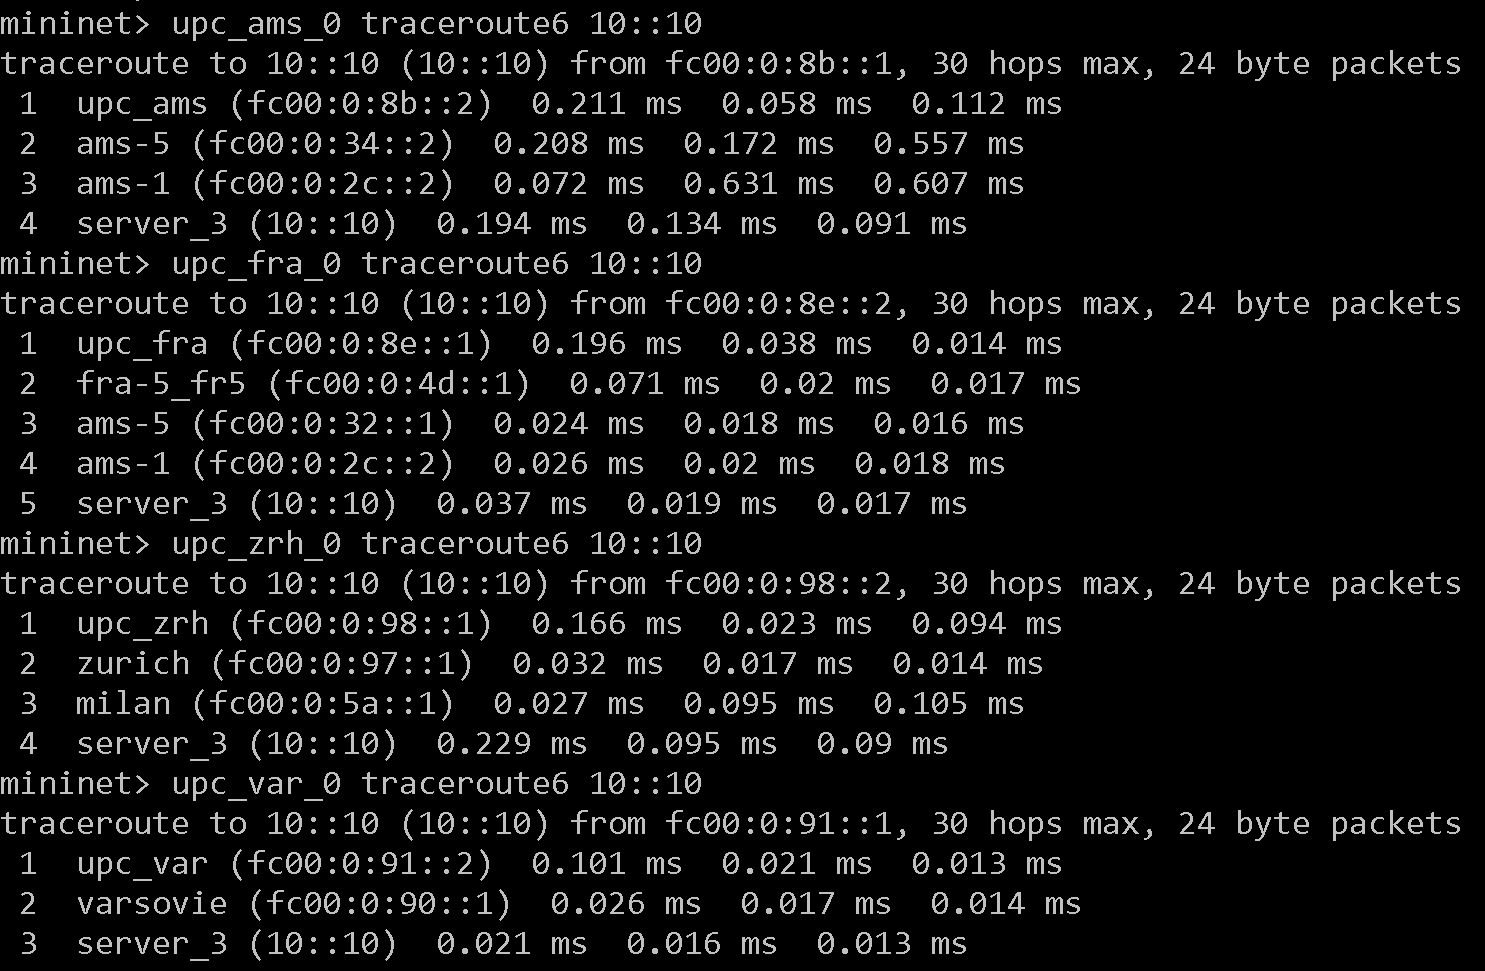
\includegraphics[width=\linewidth]{anycast_test.PNG}
    \caption{Anycast testing with traceroute}
    \label{fig:anycast_test}
\end{figure}

As shown in the figure, all hosts contacted the nearest anycast server\footnote{The server names are not always correct due to the ipmininet reverse DNS but we can identify the right server by the last router reached} as expected. 

\section{Conclusion}

As shown in this report, a good automatized simulation allows to modify and easily test different aspects of a topology configuration. 

For the OSPF part, our IP address generator helped to just define subnets instead of defining IP addresses for all routers and links. 

For the BGP aspect, the automatization was helpful to avoid duplication of codes (adding daemons and BGP configuration such as communities). 

For the security aspect, it was more difficult to add features because it was not well supported by the ipmininet library. However, lot's of research was made to understand good practices. 

For the Anycast part, the automatization allowed to automatically add servers at different places without adding links, subnets, etc. 

As shown in Sec. \ref{sec:tests}, our test were really conclusive except for the security aspect. However, now that some features are working well, it should not be too difficult to add them in our main topology. 

\addtolength{\textheight}{-10cm}   % This command serves to balance the column lengths
                                  % on the last page of the document manually. It shortens
                                  % the textheight of the last page by a suitable amount.
                                  % This command does not take effect until the next page
                                  % so it should come on the page before the last. Make
                                  % sure that you do not shorten the textheight too much.

%%%%%%%%%%%%%%%%%%%%%%%%%%%%%%%%%%%%%%%%%%%%%%%%%%%%%%%%%%%%%%%%%%%%%%%%%%%%%%%%



%%%%%%%%%%%%%%%%%%%%%%%%%%%%%%%%%%%%%%%%%%%%%%%%%%%%%%%%%%%%%%%%%%%%%%%%%%%%%%%%



\begin{thebibliography}{99}

\bibitem{ipmininet} IPMininet, \url{https://github.com/cnp3/ipmininet}
\bibitem{LINGI2142} O. Bonaventure computer course,  \url{https://uclouvain.be/cours-2020-LINGI2142.html}
\bibitem{OVHweathermap} OVH Weathermap, \url{http://weathermap.ovh.net/}
\bibitem{obo_communities} O. Bonaventure and B. Donnet, "On BGP Communities" 
\bibitem{obo_quoitin} B. Quoitin and O.Bonaventure, "A survey of the utilization of the BGP community attribute" 
\bibitem{impact_communities} T. Krenc, R. Beverly, G. Smaragdakis, "Keep your Communities Clean: Exploring the Routing Message Impact of BGP Communities" 
\bibitem{issues} IPMininet set\_local\_pref issue,  \url{https://github.com/cnp3/ipmininet/issues/99}
\bibitem{route_maps_introduction} Introduction to route maps,  \url{https://networklessons.com/cisco/ccnp-route/introduction-to-route-maps}
\bibitem{c13} \url{https://docs.umbrella.com/deployment-umbrella/docs/configure-anycast}
\bibitem{c14} \url{https://citeseerx.ist.psu.edu/viewdoc/download?doi=10.1.1.116.6367&rep=rep1&type=pdf}
\bibitem{c15} \url{http://routedo.com/posts/frr-ospf}
\bibitem{c16} BGP Anycast configuration guide, \url{https://documentation.nokia.com/html/0\_add-h-f/93-0267-HTML/7X50\_Advanced\_Configuration\_Guide/BGP\_anycast.pdf}
\bibitem{c17} BGP anycast on 2 servers. \url{https://serverius.net/bgp-anycast-dual-datacenter-using-1-ip-multiple-locations/}
\bibitem{c18} IPMininet Documentation, \url{https://ipmininet.readthedocs.io/en/latest/daemons.html#named}

\bibitem{c19} Good security practices for BGP,  \url{https://conf-ng.jres.org/2015/document_revision_2476.html?download}
\label{src_sec}

\end{thebibliography}


\end{document}
